\documentclass[../../../../main.tex]{subfiles}
\begin{document}

図のように球 $S$ に内接する球の列 $S_n$，$n=1,2,3,\cdots$ がある．
$S$ の中心 $O$ と $S_n$ の中心 $O_n$ はすべて同一平面上にあり，
$O_{n+1}$ は $S_n$ の表面上にあって，
この平面上において $O_{n+2}$ と $O_n$ は直線 $OO_{n+1}$ に関して互いに反対側にある．
また $S$ の半径は $a$，$S_n$ の半径は $\displaystyle\frac{a}{2^n}$ である．
このとき，

\begin{figure}[htbp]
  \centering
  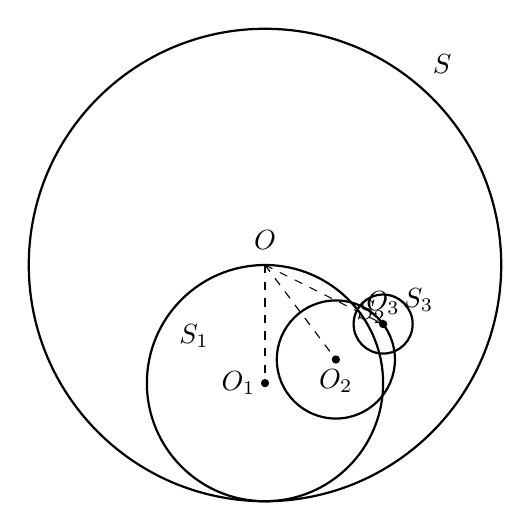
\begin{tikzpicture}[scale=1.5, >=stealth]
    \coordinate (O) at (0,0);
    \draw[thick] (O) circle (2.0);
    \node[above=2pt] at (O) {$O$};
    \node at (1.5, 1.7) {$S$};

    \coordinate (O1) at (0, -1.0);
    \draw[thick] (O1) circle (1.0);
    \fill (O1) circle (1pt) node[left] {$O_1$};
    \node at (-0.6, -0.6) {$S_1$};

    \coordinate (O2) at (0.6, -0.8);
    \draw[thick] (O2) circle (0.5);
    \fill (O2) circle (1pt) node[below] {$O_2$};
    \node at (0.9, -0.4) {$S_2$};

    \coordinate (O3) at (1.0, -0.5);
    \draw[thick] (O3) circle (0.25);
    \fill (O3) circle (1pt) node[above] {$O_3$};
    \node at (1.3, -0.3) {$S_3$};

    \draw[dashed] (O) -- (O1);
    \draw[dashed] (O) -- (O2);
    \draw[dashed] (O) -- (O3);
  \end{tikzpicture}
\end{figure}

\begin{enumerate}
  \item $S_n$ と $S_{n+1}$ の共通部分の体積 $v_n$ を求めよ．
  \item $m=1,2,3,\cdots$ に対して，$\displaystyle V_m=\sum_{n=1}^m v_n$ とおくとき，
  $\displaystyle V=\lim_{m\to\infty}V_m$ を求めよ．
\end{enumerate}

\end{document}
